\documentclass[a4paper,11pt,openright]{report}
\usepackage[utf8]{inputenc}
\usepackage[italian]{babel}
\usepackage{amssymb}
\usepackage{amsmath}
\usepackage{amsthm}
\usepackage{float}
\usepackage{afterpage}
\usepackage{graphicx}
\usepackage[toc,page]{appendix}
\usepackage{biblatex}
%\usepackage[margin=1in]{geometry}
\renewcommand{\appendixtocname}{Appendice}
\renewcommand{\appendixpagename}{Appendice}
\newtheorem{teo}{Teorema}[section]
\newtheorem{lemma}[teo]{Lemma}
\newtheorem{osservazione}[teo]{Osservazione}
\newtheorem{esempio}[teo]{Esempio}
\newtheorem{ipotesi} [teo]{Ipotesi}
\newtheorem{notazione}[teo]{Notazione}
\newtheorem{corollario}[teo]{Corollario}
\newtheorem{proposizione}[teo]{Proposizione}
\newtheorem{euristica}[teo]{Euristica}
\newtheorem{definizione}[teo]{Definizione}
\newtheorem{notabene}[teo]{N.B.}

\newcommand\blankpage{
	\null
	\thispagestyle{empty}
	\newpage
	}



\begin{document}

\chapter*{Numerical Study with T = 1, n = 3, sigma = 0.3}

\section{MC with $10^6$ particels}
Euler - Monte Carlo execution time:  127.859375 \\
Euler - Monte Carlo error:  0.001480500282752356

\begin{figure}[H]
\centering
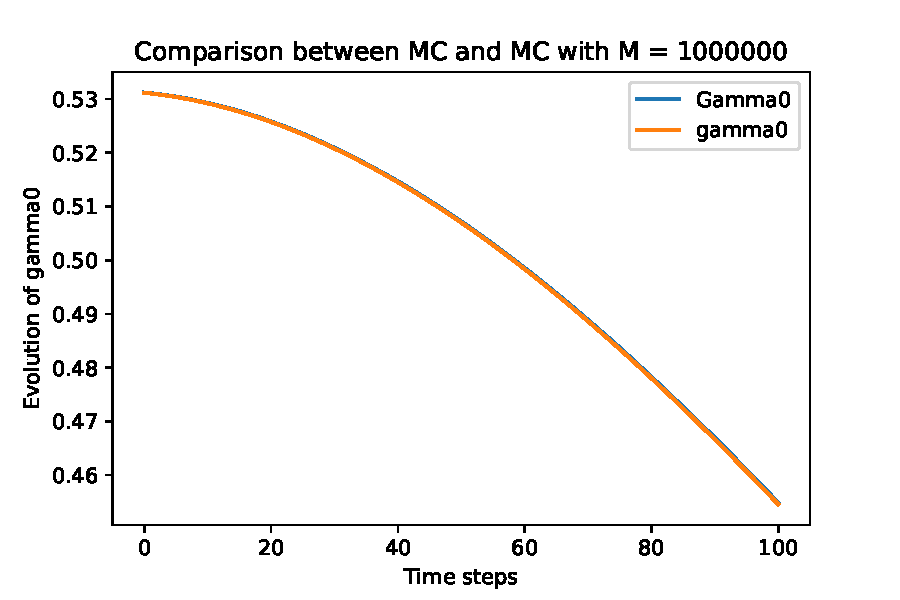
\includegraphics[width=0.9\textwidth]{gamma0 MC = 1000000.pdf}
\end{figure}
\begin{figure}[H]
\centering
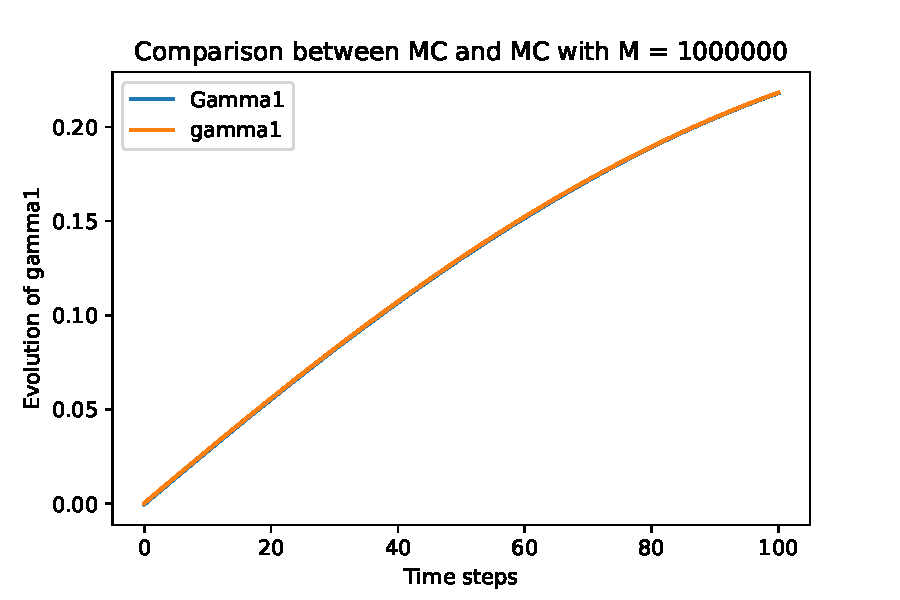
\includegraphics[width=0.9\textwidth]{gamma1 MC = 1000000.pdf}
\end{figure}
\begin{figure}[H]
\centering
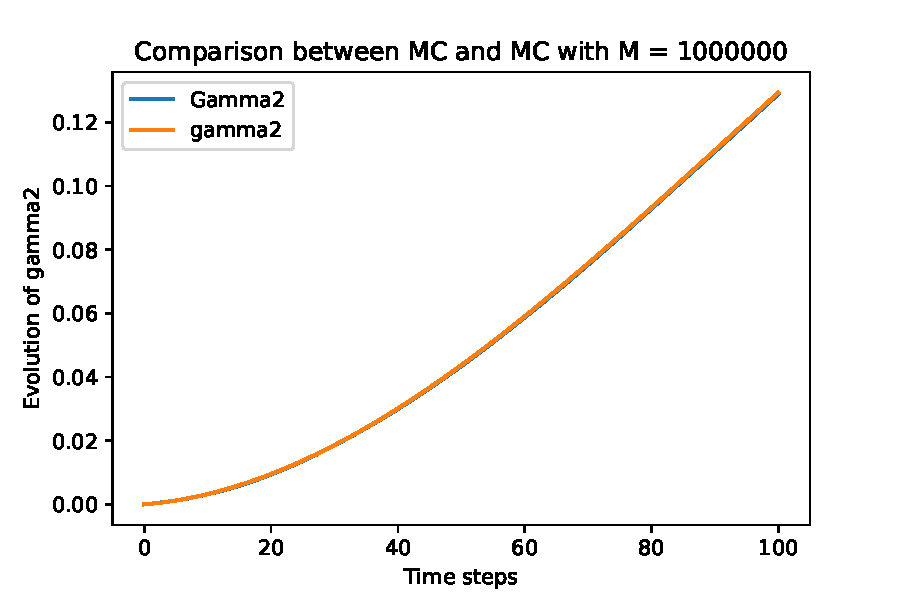
\includegraphics[width=0.9\textwidth]{gamma2 MC = 1000000.pdf}
\end{figure}
\begin{figure}[H]
\centering
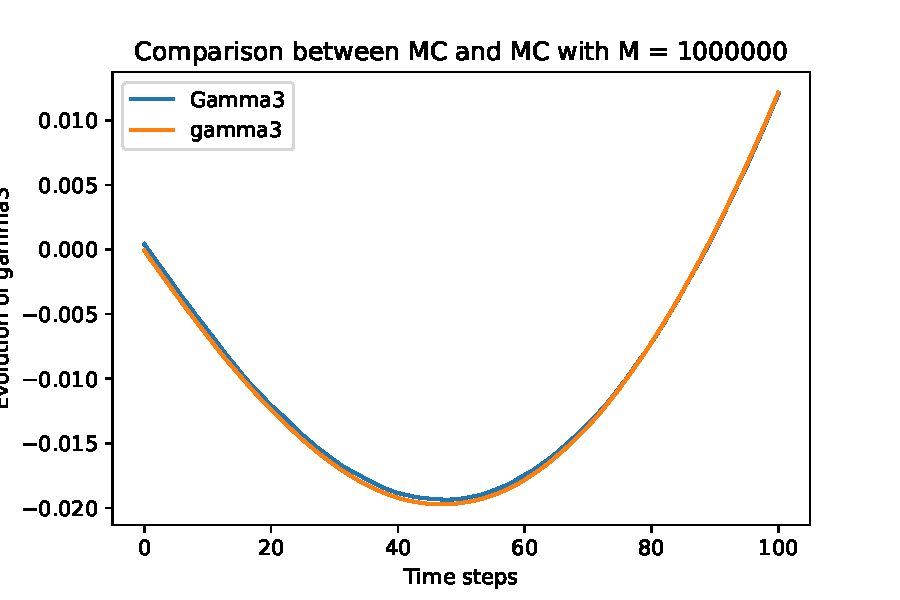
\includegraphics[width=0.9\textwidth]{gamma3 MC = 1000000.pdf}
\end{figure}
\begin{figure}[H]
\centering
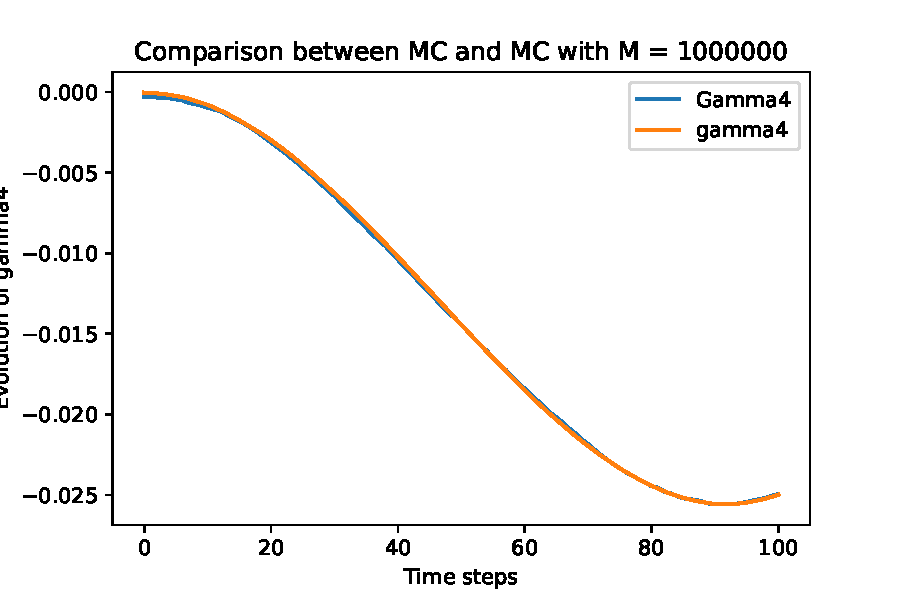
\includegraphics[width=0.9\textwidth]{gamma4 MC = 1000000.pdf}
\end{figure}
\begin{figure}[H]
\centering
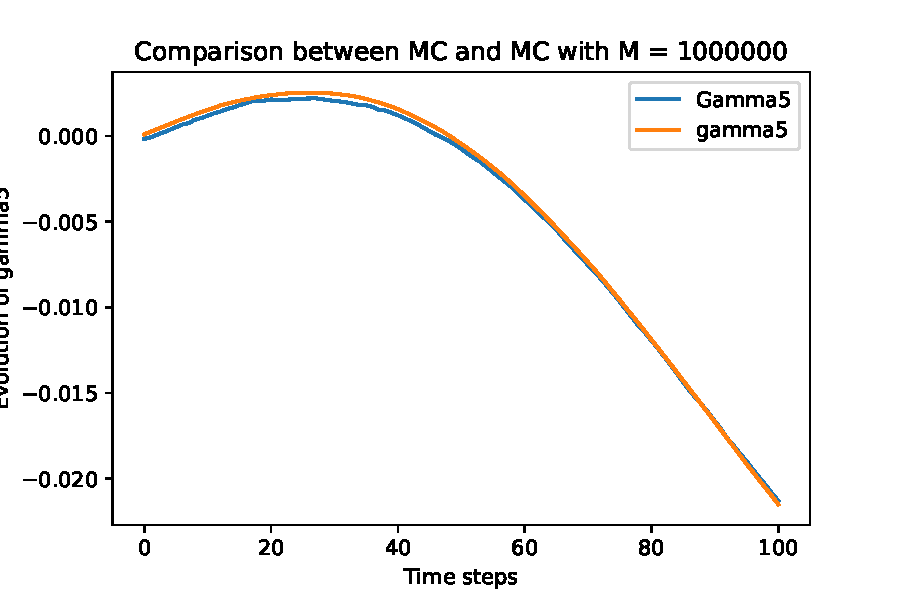
\includegraphics[width=0.9\textwidth]{gamma5 MC = 1000000.pdf}
\end{figure}
\newpage

\section{MC with $10^5$ particels}
Euler - Monte Carlo execution time:  24.96875 \\
Euler - Monte Carlo error:  0.0056881373542012215

\begin{figure}[H]
\centering
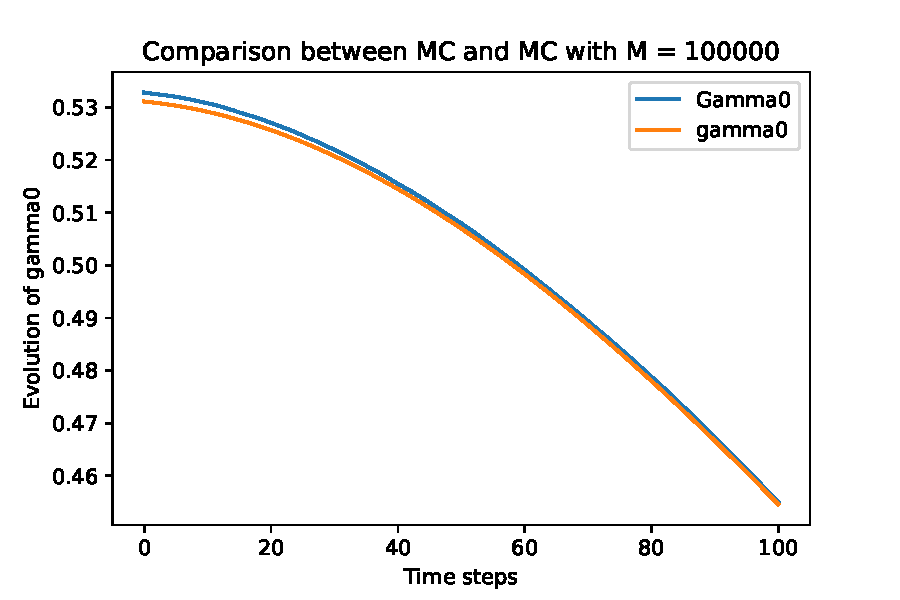
\includegraphics[width=0.9\textwidth]{gamma0 MC = 100000.pdf}
\end{figure}
\begin{figure}[H]
\centering
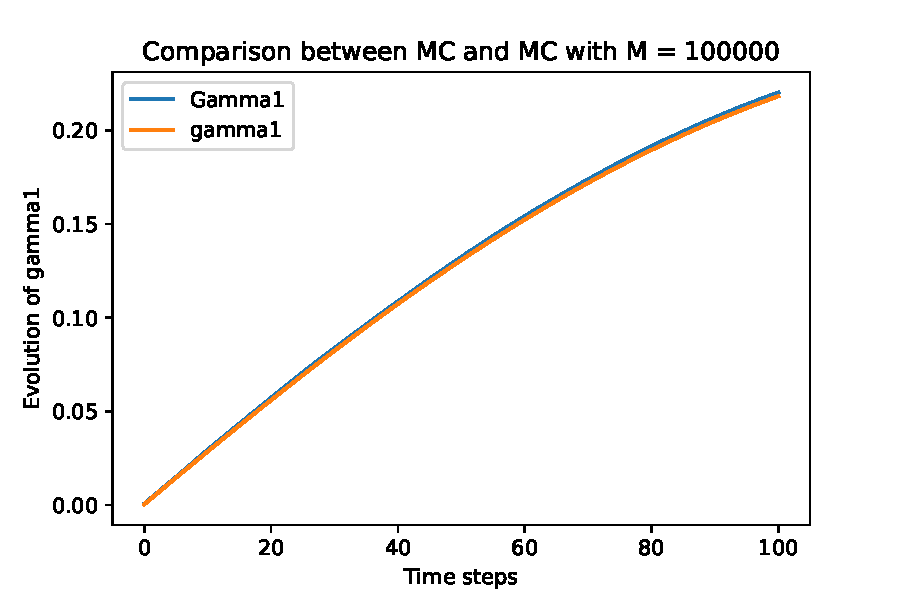
\includegraphics[width=0.9\textwidth]{gamma1 MC = 100000.pdf}
\end{figure}
\begin{figure}[H]
\centering
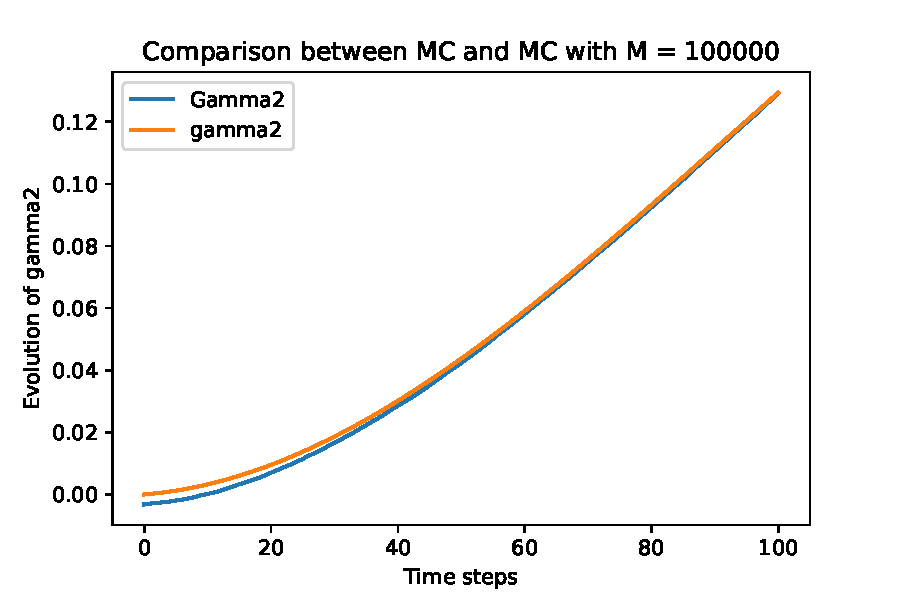
\includegraphics[width=0.9\textwidth]{gamma2 MC = 100000.pdf}
\end{figure}
\begin{figure}[H]
\centering
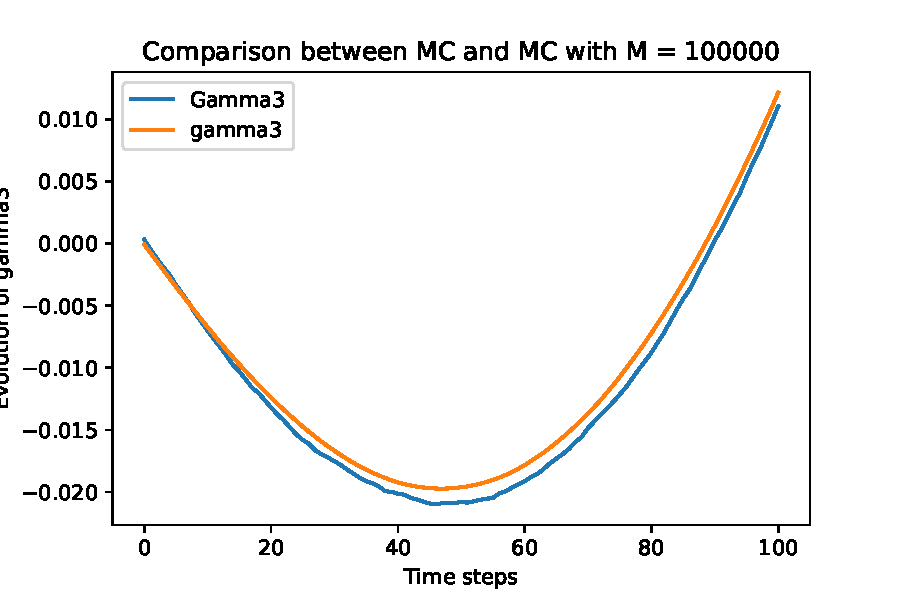
\includegraphics[width=0.9\textwidth]{gamma3 MC = 100000.pdf}
\end{figure}
\begin{figure}[H]
\centering
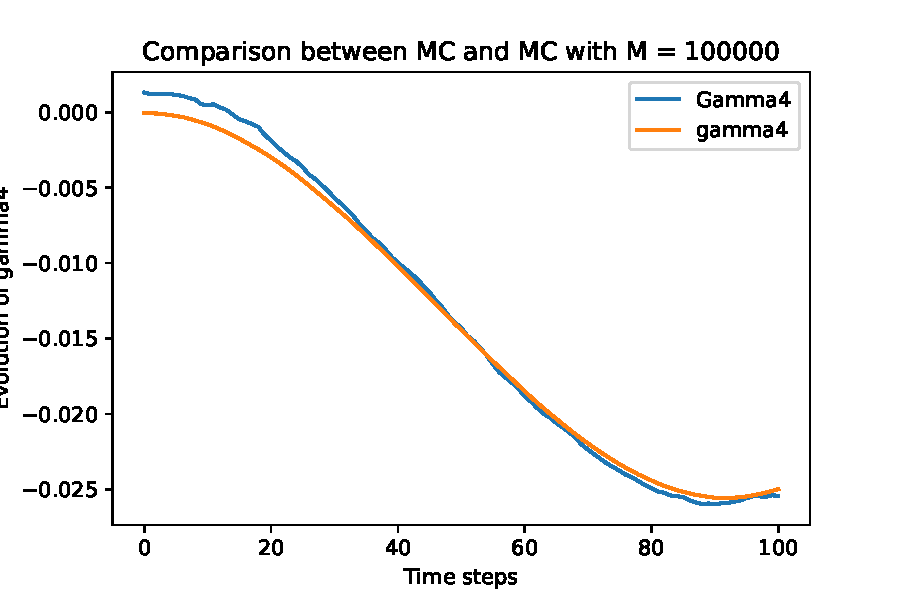
\includegraphics[width=0.9\textwidth]{gamma4 MC = 100000.pdf}
\end{figure}
\begin{figure}[H]
\centering
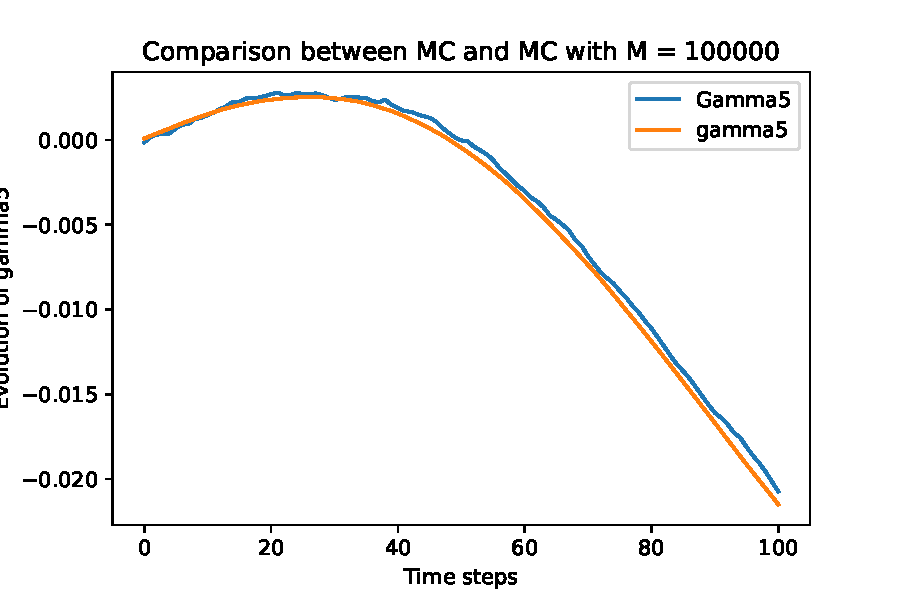
\includegraphics[width=0.9\textwidth]{gamma5 MC = 100000.pdf}
\end{figure}
\newpage

\section{MC with $10^4$ particels}
Euler - Monte Carlo execution time:  2.484375 \\
Euler - Monte Carlo error:  0.011473528868816807

\begin{figure}[H]
\centering
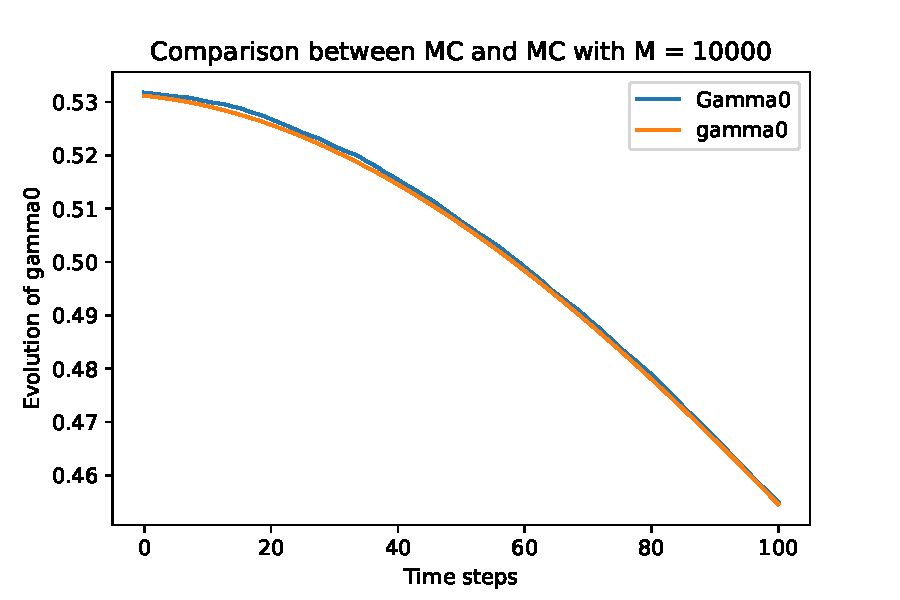
\includegraphics[width=0.9\textwidth]{gamma0 MC = 10000.pdf}
\end{figure}
\begin{figure}[H]
\centering
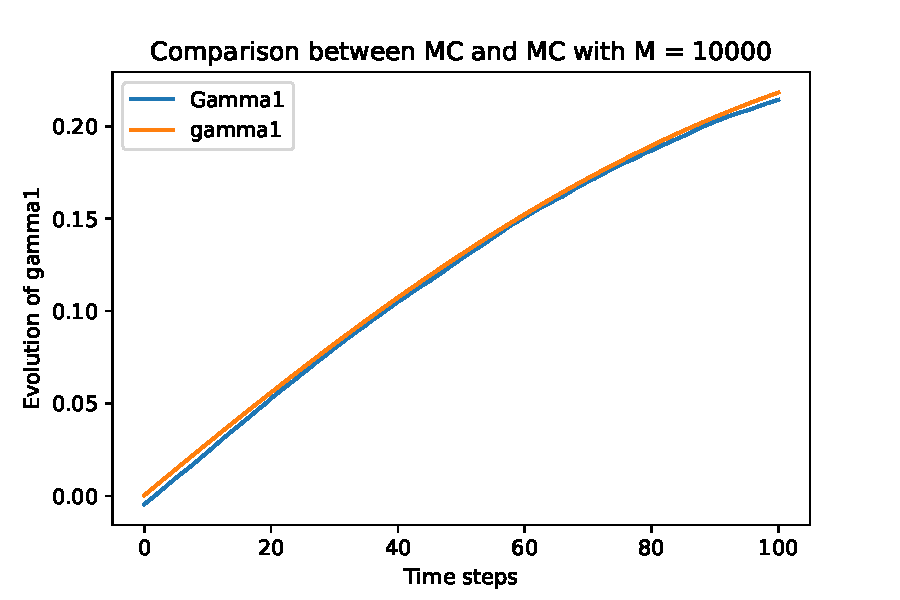
\includegraphics[width=0.9\textwidth]{gamma1 MC = 10000.pdf}
\end{figure}
\begin{figure}[H]
\centering
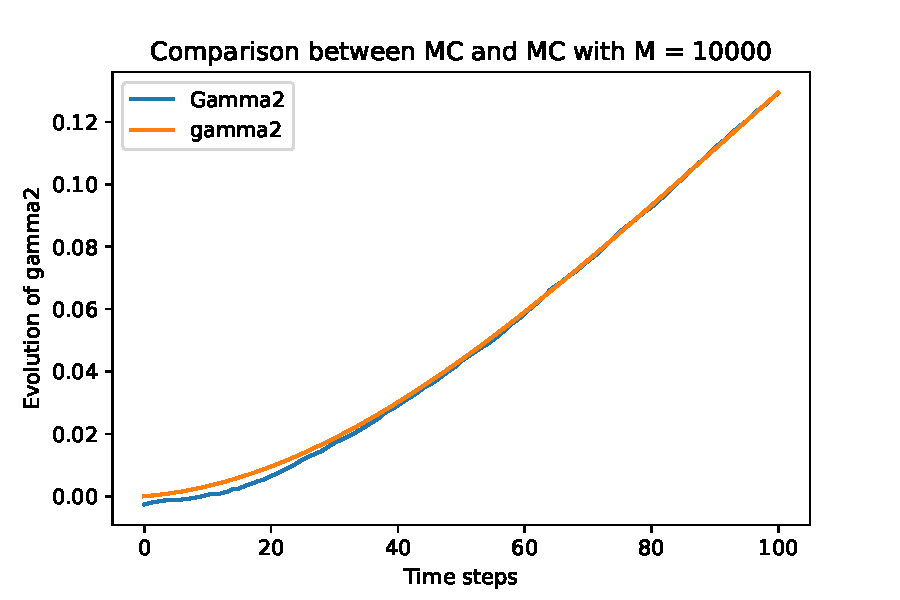
\includegraphics[width=0.9\textwidth]{gamma2 MC = 10000.pdf}
\end{figure}
\begin{figure}[H]
\centering
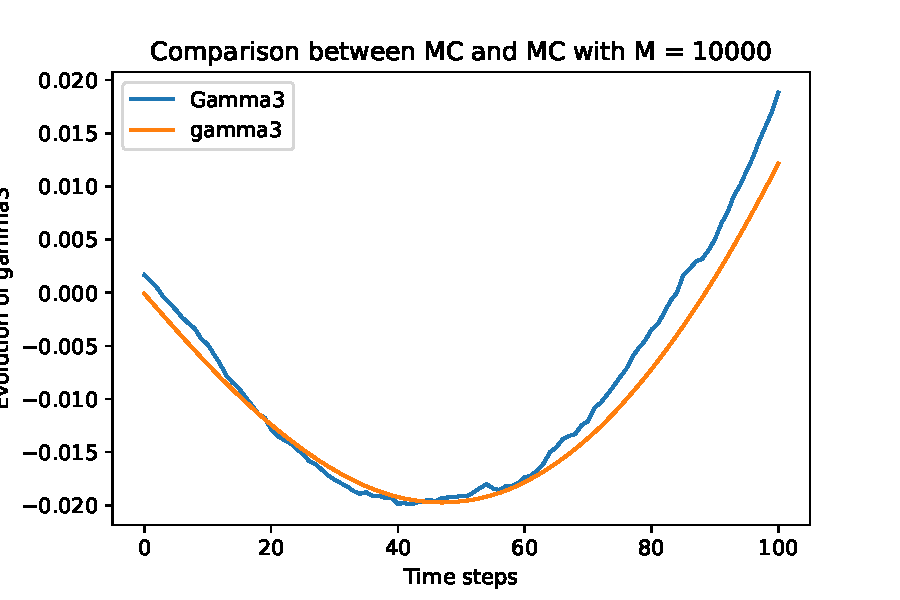
\includegraphics[width=0.9\textwidth]{gamma3 MC = 10000.pdf}
\end{figure}
\begin{figure}[H]
\centering
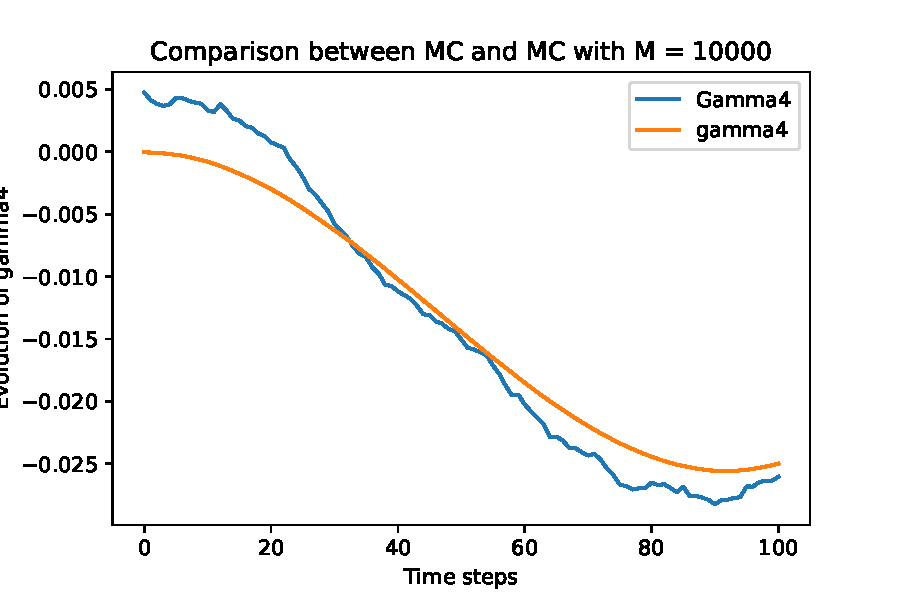
\includegraphics[width=0.9\textwidth]{gamma4 MC = 10000.pdf}
\end{figure}
\begin{figure}[H]
\centering
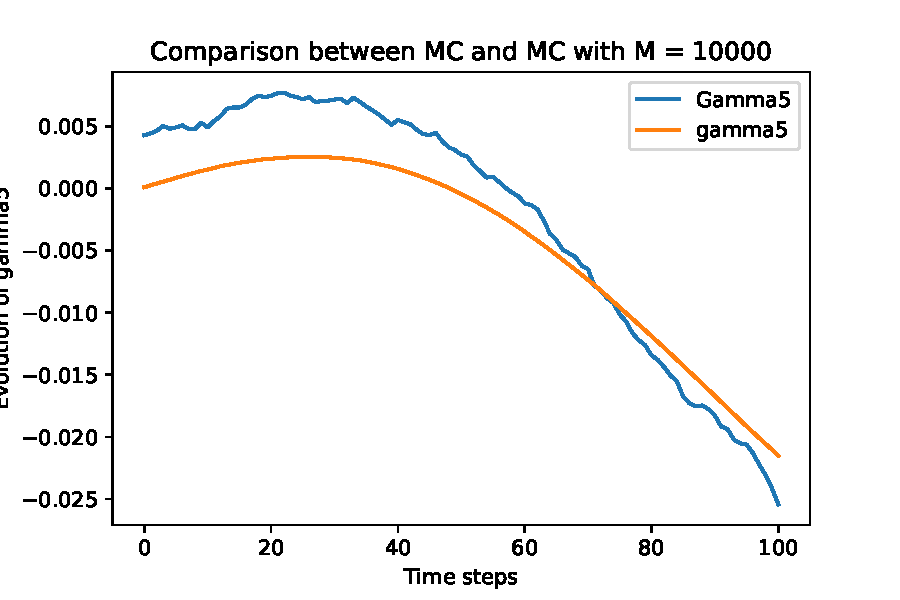
\includegraphics[width=0.9\textwidth]{gamma5 MC = 10000.pdf}
\end{figure}
\newpage

\section{SGD with M = 100}
SGD execution time: 13.65625 \\
SGD steps: 150

\begin{figure}[H]
\centering
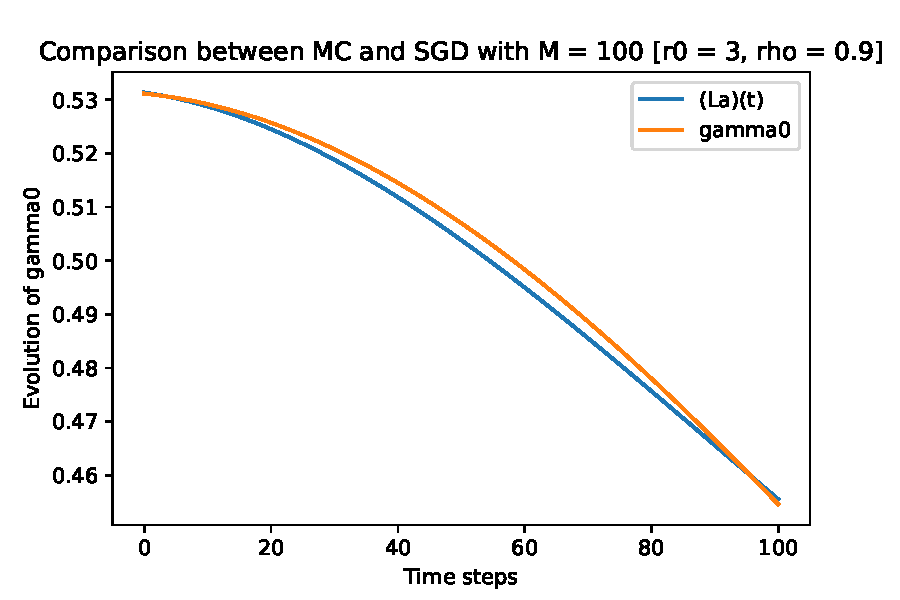
\includegraphics[width=0.9\textwidth]{gamma0 SGD 100.pdf}
\end{figure}
\begin{figure}[H]
\centering
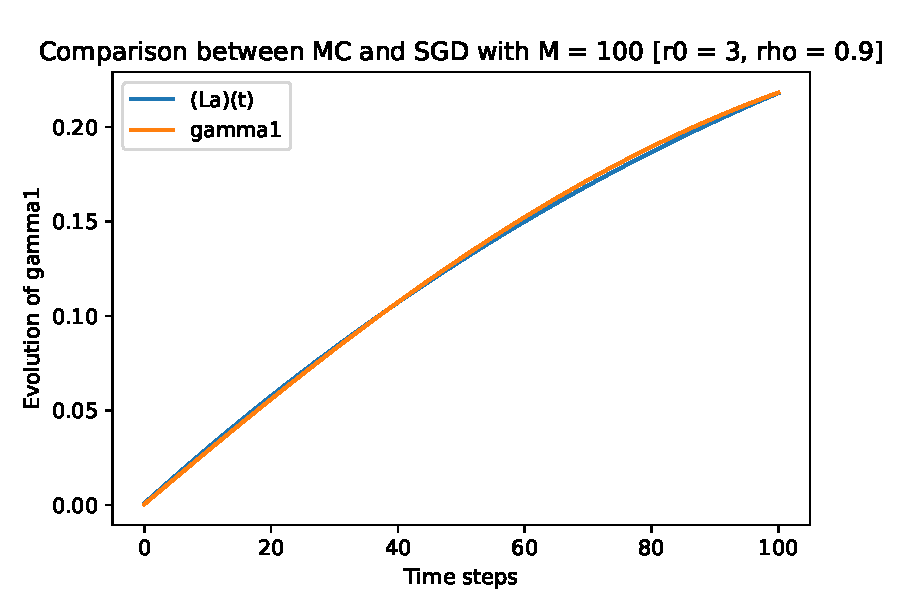
\includegraphics[width=0.9\textwidth]{gamma1 SGD 100.pdf}
\end{figure}
\begin{figure}[H]
\centering
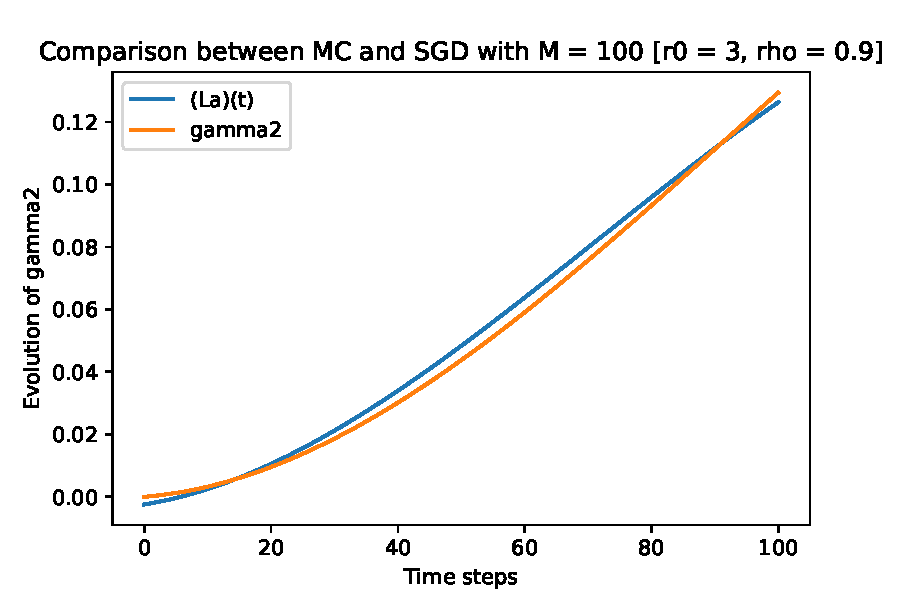
\includegraphics[width=0.9\textwidth]{gamma2 SGD 100.pdf}
\end{figure}
\begin{figure}[H]
\centering
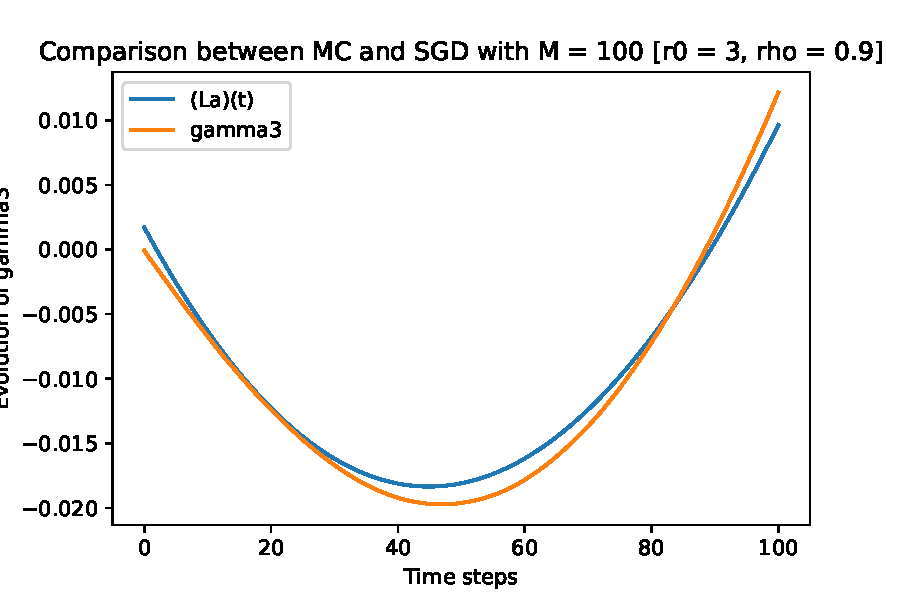
\includegraphics[width=0.9\textwidth]{gamma3 SGD 100.pdf}
\end{figure}
\begin{figure}[H]
\centering
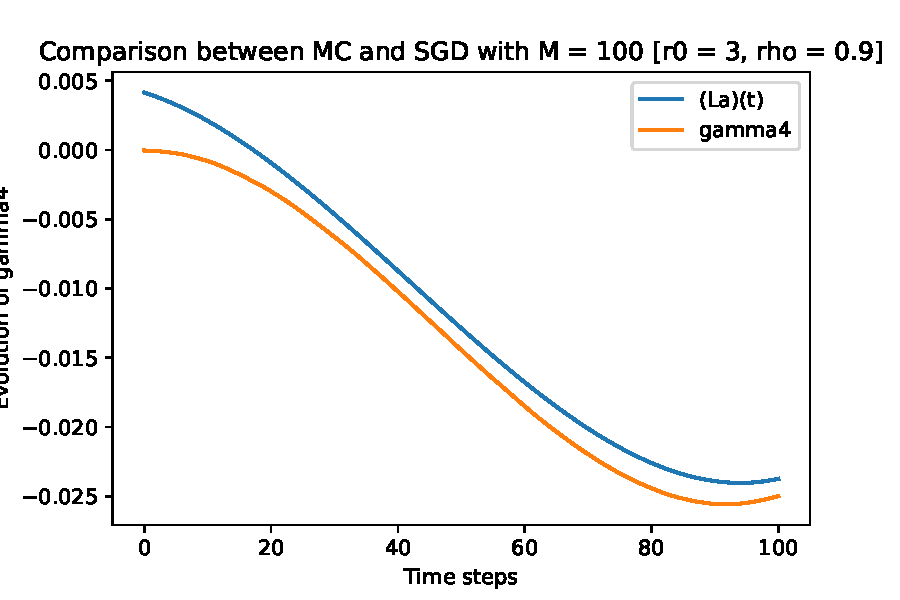
\includegraphics[width=0.9\textwidth]{gamma4 SGD 100.pdf}
\end{figure}
\begin{figure}[H]
\centering
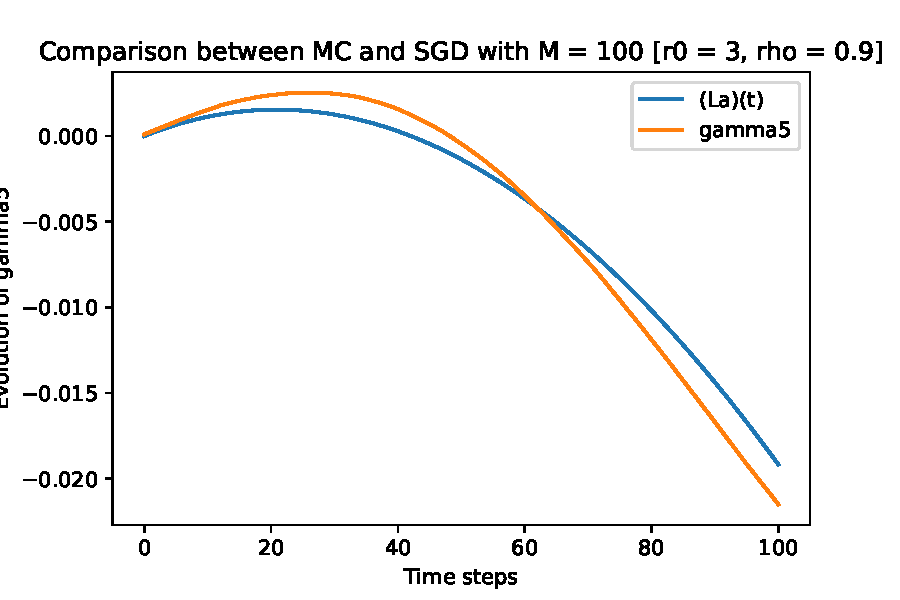
\includegraphics[width=0.9\textwidth]{gamma5 SGD 100.pdf}
\end{figure}

\section{SGD with M = 1000}
SGD execution time: 42.609375 \\
SGD steps: 60

\begin{figure}[H]
\centering
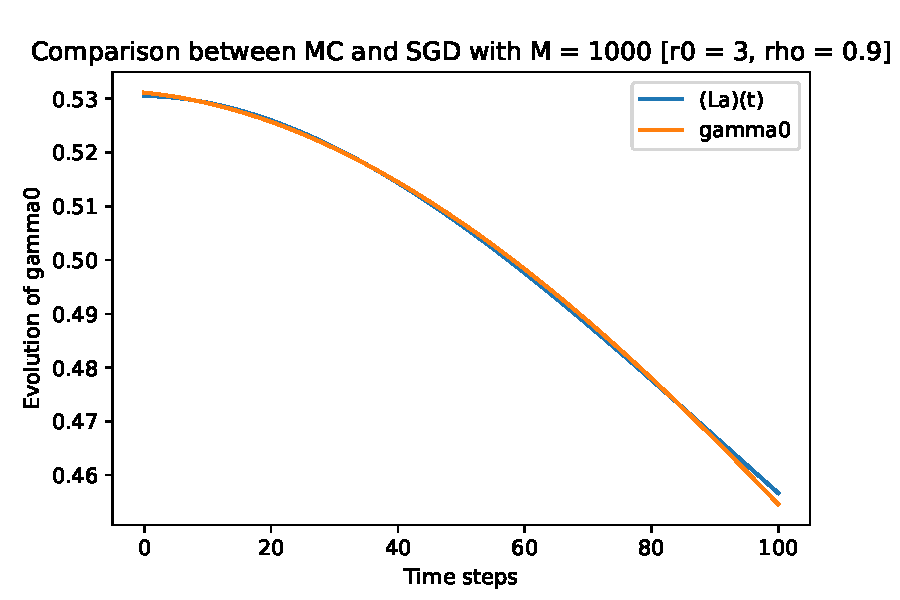
\includegraphics[width=0.9\textwidth]{gamma0 SGD 1000.pdf}
\end{figure}
\begin{figure}[H]
\centering
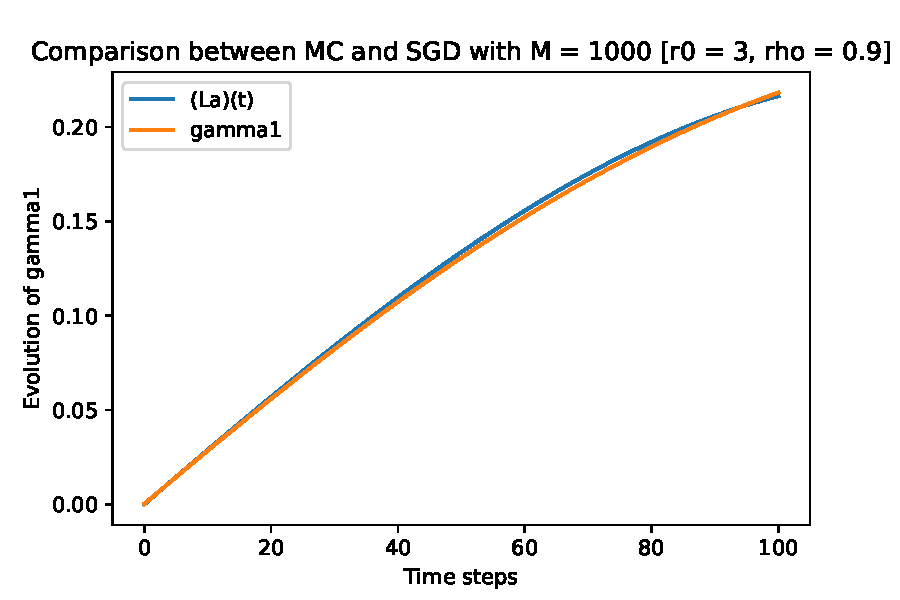
\includegraphics[width=0.9\textwidth]{gamma1 SGD 1000.pdf}
\end{figure}
\begin{figure}[H]
\centering
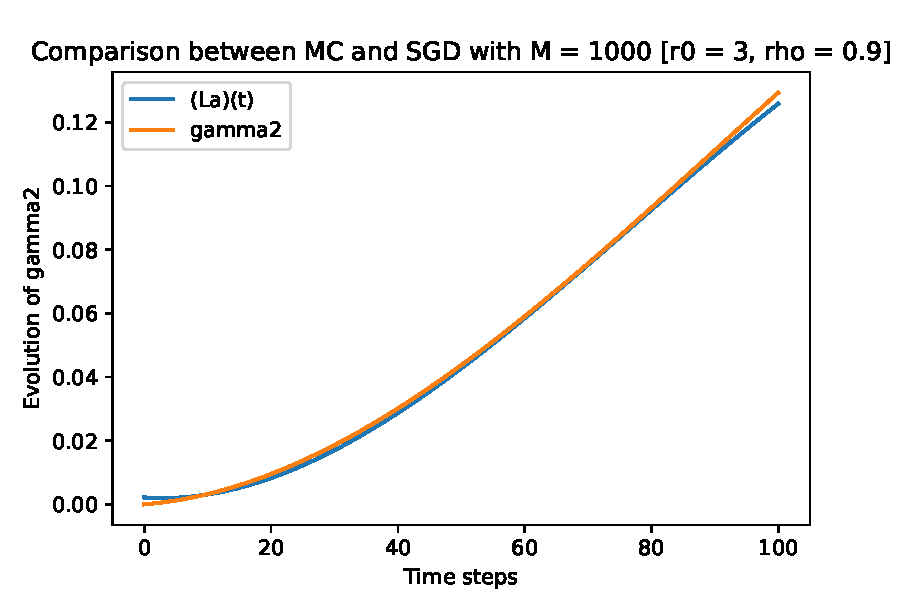
\includegraphics[width=0.9\textwidth]{gamma2 SGD 1000.pdf}
\end{figure}
\begin{figure}[H]
\centering
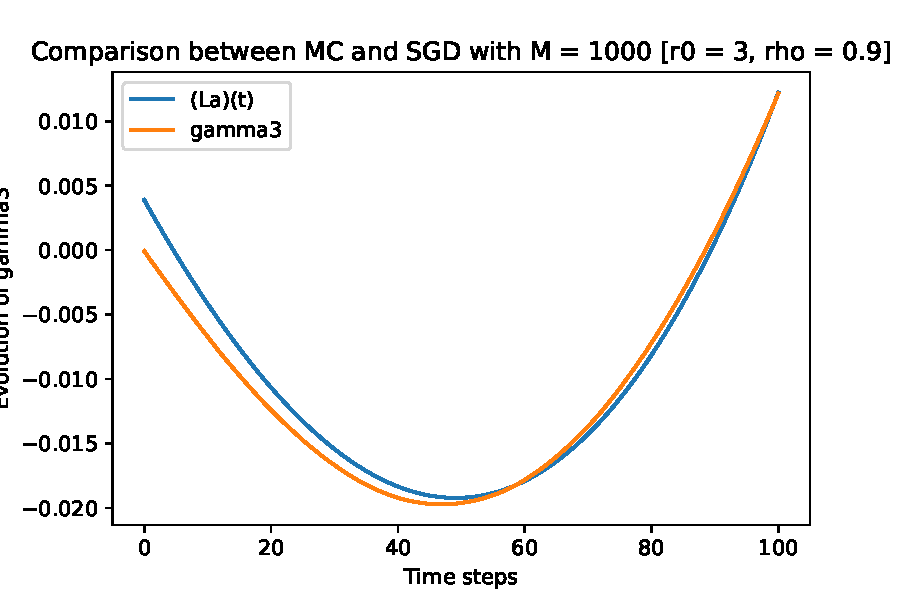
\includegraphics[width=0.9\textwidth]{gamma3 SGD 1000.pdf}
\end{figure}
\begin{figure}[H]
\centering
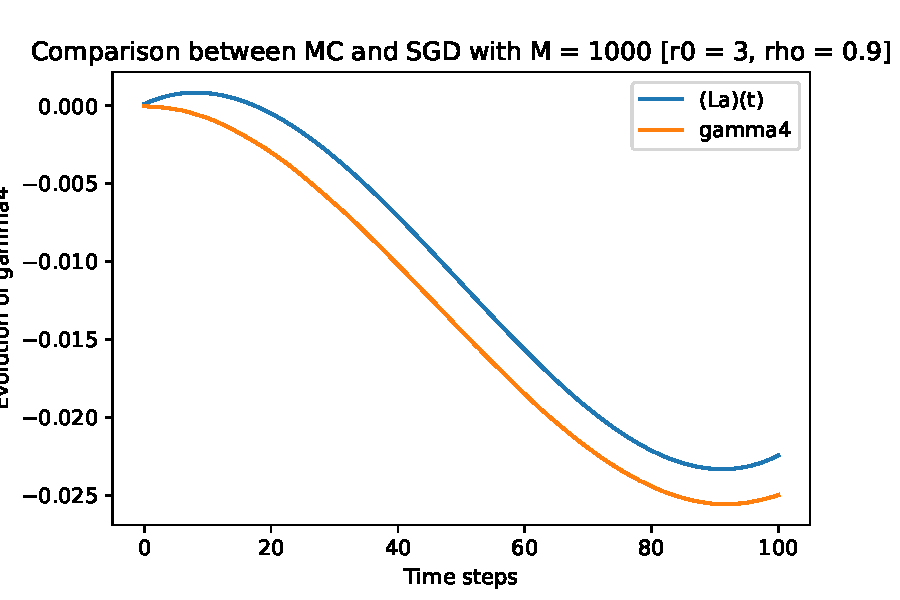
\includegraphics[width=0.9\textwidth]{gamma4 SGD 1000.pdf}
\end{figure}
\begin{figure}[H]
\centering
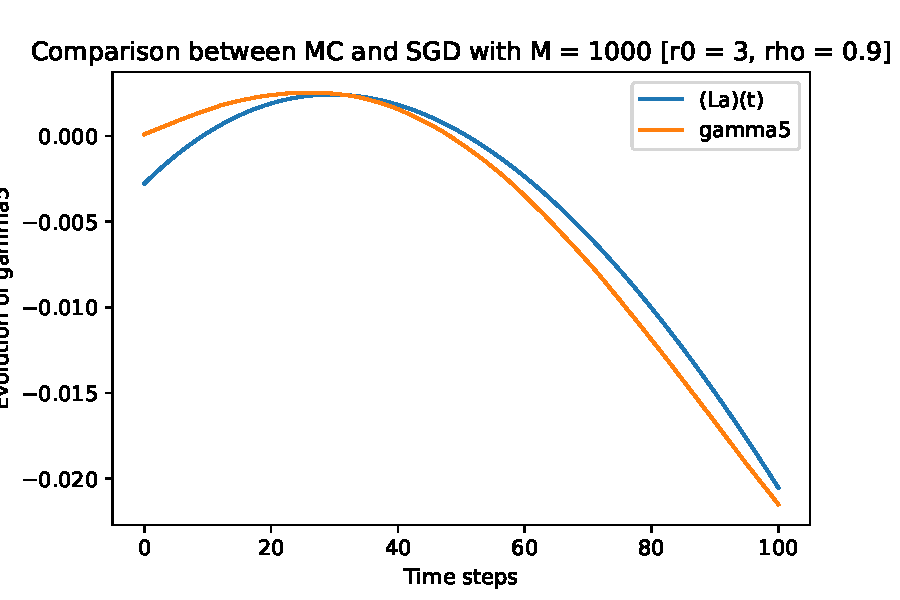
\includegraphics[width=0.9\textwidth]{gamma5 SGD 1000.pdf}
\end{figure}

\newpage
\section{Tables}
\begin{table}[H]
\centering
\addtolength{\leftskip}{-1.5cm}
\addtolength{\rightskip}{-1.5cm}
\begin{tabular}{|c|lllll|}
\hline
$ $ & MC $10^6$ & MC $10^5$ & MC $10^4$ & SGD $100$ & SGD $1000$\\
\hline
time & 127.86 & 24.97 & 2.48 & 13.66 & 42.61 \\

error & 0.0015 & 0.0057 & 0.011 & 0.001 & 0.001 \\

steps & / & / & / & 150 & 60 \\

\hline
\end{tabular}
\caption{Comparisons}
\end{table}


\end{document}
